\chapter{Polarization-entangled photons}
\labelChapter{polarization_entangled_photons}

\begin{epigram}{\textit{Asher Peres, Quantum Theory: Concepts and Methods}}
    \enquote{Quantum phenomena do not occur in a Hilbert space. They occur in a laboratory.} 
\end{epigram}

\section{Introduction: Non-separability in the laboratory}
\labelChapter{C4_introduction}

\lettrine[lines=3]{I}{n} the introductory chapter we have described various linear optical elements and how information can be encoded and subsequently measured in the polarization \acs{DOF} of a single photon. As the avid reader (or by the title of this thesis) might have suspected, much of the appeal of such optical systems comes about from their potential applications to quantum information processing tasks. In this particular chapter, we steer towards this direction and consider this use of polarization-entangled pairs of photons generated \via a nonlinear process called \acs{SPDC}, with the polarization of a single-photon as a substrate for a quantum bit. Multi-qubit states that possess non-classical correlations have been realized in a variety of, and often exotic optical systems, but in this regard perhaps, the most readily available and controllable source of entanglement arises from polarization-entangled photons. This is in part attested by their ubiquitous use; for demonstrations of Shor's algorithm from the first half of thesis (see ~\refChapterOnly{quantum_prime_factorization}); after the pioneering work on a spin-$\nicefrac{1}{2}$ nuclei system~\cite{Vandersypen_2001}, have been realized on single-photonic architectures making use of polarized-entangled photons~\cite{Lu_2007,Lanyon_2007,Lopez_2012} and other sundry tasks; including state-preparation in measurement-based/one-way quantum computing~\cite{Lu_2006, Kiesel_2005, Park_2007, Vallone_2008, Tokunaga_2008}, algorithms~\cite{Walther_2005, Prevedel_2007, Chen_2007} and quantum communication protocols~\cite{Kiesel_2007, Gaertner_2008, Schmid_2010, Bell_2014}. 

\bigskip
\noindent
Needless to say, the commonality among all these demonstrations is the central role of entanglement, which necessitates the need for a complete characterization of such entangled states in such applications. In earlier pioneering work of this kind, qualitative arguments for the presence of entanglement were made in the way of violation of Bell-type inequalities from fringe visibility measurements being above a certain threshold~\cite{Kwiat_1995, Kwiat_1999}. Such measurements gave qualitative evidence for the existence of non-classical correlations in a given experiment, not consistent with any local hidden-variable theory~\cite{Bell_1964,CHSH_1969,GHZ_2007}. 

\bigskip
\noindent
A violation of Bell-type inequalities is often considered an excellence indicator of the presence of entanglement in a pure two-qubit system; alas, despite its experimental convenience, it is not a true measure of entanglement\footnote{Ref.~\cite{Munro_2001} shows that in general, it is not possible to discern the degree of entanglement (a quantifiable measure) in a state \via an inference from a violation of Bell-type inequality}. 

\clearpage
\noindent
A more thorough characterization of polarization-entangled photons is through \gls{QST}~\cite{Hradil_1997, James_2001}. From a set of measurements performed on an ensemble of identically prepared quantum states, a maximum likelihood estimate of the density matrix of the polarization-entangled photon state is obtained, and from which physical quantities of interest such as fidelity, purity and concurrence can be derived.

\section{Experimental design}
\labelSection{C4_experimental_design}

In the experiment that we will describe in this chapter, we endeavour to generate and characterize a photonic three-qubit maximally entangled state\footnote{Maximally entangled state has a maximum entropy of entanglement for each of its bipartitions. For a two qubits, the Bell states are examples of maximally-entangled states.} first studied by \gls{GHZ} and thus bears their name. The experimental procedure is conceptually simple to describe: A two-photon, two-qubit polarized-entangled state is generated from a \acs{SPDC} and appropriately characterized with quantum state tomography. Once characterized and optimized, this state is enlarged by using the path (momentum) \acs{DOF} of one of the photons to a three-qubit polarization and path entangled \acs{GHZ} state, locally equivalent to a graph state~\cite{Raussendorf_2003}. Encoding a quantum bit on a separate \acs{DOF} on one of the polarization-entangled photons is motivated by two main reasons.

\begin{itemize}
	\item[\emph{Primo}] Experimental convenience: Having additional photons (generated by another \acs{SPDC} process) in an experimental setup of this kind would necessitate additional tabletop linear optical components \ie mirrors, wave plates, beam splitters, filters, polarizers, etc. The end goal of the experiment is to eventually carry out remotely controllable measurements on the generated state, thus it is preferable to have fewer moving parts. 

	\item[\emph{Secondo}] Practicality: \acs{SPDC} is a probabilistic process, that is, for every photon incident on the crystal, with some probability $p$, it will down convert to a polarization-entangled photon-pair, and the probability $p$ is typically low, on the order of $\lesssim 1\%$~\cite{Kok_2007}. Thus having an additional two photons produced in our experimental setup would occur with even lower probability $p^2$ (assumption of independence of the two events), and would also alter the coincidence counting electronics; typically one has to allow a long coincidence window to observe multiple low probability events of this kind\footnote{In Ref.\cite{Lu_2006}, a six-photon, six-qubit polarized-entangled state was produced with three \acs{SPDC} processes occurring in succession,and six-fold coincidence events (${\sim p^3}$) were accumulated over a three hour coincidence window.}.
\end{itemize}

\noindent
Similarly, once this state is generated, we appropriately characterize it. Reconstructing the density matrix of a three-qubit state would necessitate a full tomographic analysis, which for a three-qubit state would require $64$ measurement settings~\cite{Resch_2005}. However, a \acs{GHZ} state is locally equivalent to another three-qubit state that is a member of a special class of states, called graph states~\cite{Hein_2004,Raussendorf_2003}. What is peculiar to graph states is that they are completely described by their so-called stabilizer operators, which provide an experimentally economical way to discern the presence of entanglement and a lower bound for the fidelity of the generated state by way of evaluating their expectation values~\cite{Toth_2005}.

\bigskip
\noindent
Once characterized, we proceed to automate the experimental calibration and measurement procedures. This is achieved by having the relevant linear optical components in our experimental setup, all connected to a centralized and remotely accessible server that mediates the control of the optical components. 

\clearpage

\begin{figure*}[t!]
  \centering
  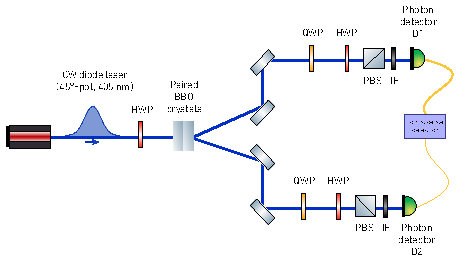
\includegraphics[width=1.0\textwidth]{experiment_1.pdf}%
  \caption[Experimental setup for generation and measurement of a two-photon two-qubit polarization-entangled Bell state.]{Experimental setup for generation and measurement of a two photon two-qubit Bell state. \gls{HWP}, \gls{QWP}, \gls{BBO}, \gls{PBS}, \gls{NPBS} and \gls{IF}. A photon pair is created whenever a laser pump photon with \SI{405}{nm} wavelength is incident on the paired \acs{BBO} crystals cut for type-I \acs{SPDC}, generating photons at \SI{810}{nm}. Each photon is guided by a set of mirrors to a \acs{QWP}, \acs{HWP}, and \acs{PBS} which are used to perform polarization measurements of the quantum state. Finally, each photon is sent to an \acs{IF} at \SI{800}{nm} with a bandwidth of \SI{40}{nm} and collected by a \gls{SMF} and sent to a photon detector. Each photon detector produces an electronic signal and sends it to the coincidence counting electronics, which count the signals that arrive simultaneously.}
  \labelFigure{experiment_1}
\end{figure*}

\noindent
With accessibility in mind, we designed a proof-of-concept mobile app that provides a graphical user interface to communicate with the server, which permits the user to specify an experiment with arbitrary (allowed) measurement settings and retrieve their experimental results. The rest of this chapter is dedicated to the filling in the details and describing the experimental design and subsequently, results from the experiments.

\bigskip
\noindent
The main goal of the initial stage of the experiment was to characterize the polarization-entangled two-photon two-qubit state from a \acs{SPDC} source using full quantum state tomography. To perform full quantum state tomography, we used the techniques and tools described in Ref.~\cite{James_2001}. We begin by describing the various components of the experimental apparatus shown in ~\refFigureOnly{experiment_1} --- A laser and \acs{SPDC} source, measurement apparatus, photon collection optics, and coincidence detection electronics. The \acs{SPDC} source used was two concatenated \SI{5}{\milli\meter} $\times$ \SI{5}{\milli\meter} $\times$ \SI{0.5}{\milli\meter} \gls{BBO} crystals cut for type-I phase matching, with their two optical axes aligned in perpendicular planes. 

\bigskip
\noindent
When this source is pumped with a vertically polarized pump beam, due to type-I phase-matching, down-conversion will occur in the first crystal producing  horizontally polarized energy-degenerate, non-collinear photon pairs. Similarly, a horizontally polarized pump beam will stimulate type-I down-conversion in the second crystal, generating energy-degenerate photon pairs. A diagonally polarized laser is likely to equally stimulate down-conversion in both crystals~\cite{Kwiat_1999}. Photons in the spatially overlapping regions, diametrically opposed (due to momentum conservation) on the two light cones, will be in the state $(\ket{H_1,H_2} + e^{i\phi}\ket{V_1,V_2})/\sqrt{2}$ as illustrated in~\refFigureOnly{two_type_I}. A main condition here is that the spatial modes of a given pair must have a significant overlap~\cite{Kwiat_1999}. Our \acs{SPDC} source is pumped with a \gls{CW} blue laser\footnote[][-55pt]{We keep our power relatively low, as high power pumps are known to stimulate double pair emissions~\cite{Weinfurter_2001,Fulconis_2007}, which degrade the single-photon quality. Our laser pump operates at a power of $\sim$\SI{50}{\milli\watt}) for every experiment we conducted unless stated otherwise.}, to produce frequency-degenerate photon pairs at a wavelength of \SI{810}{\nano\meter}, emitted onto a light cone with an (full) opening angle of $6^{\circ}$. 

\clearpage
\begin{figure}[h]
	\centering
	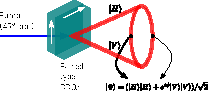
\includegraphics[width=\textwidth]{type-I-SPDC.pdf}
	\caption[Two paired \acs{BBO} ($\beta$-barium borate) crystals cut for type-I phase matching.][-15pt]{Two paired \acs{BBO} ($\beta$-barium borate) crystals cut for type-I phase matching as a source of entangled photons. For every pump photon, the photon pairs emerge from the crystal at a fixed from the pump photon thus creating a cone around the direction of the pump photon. Photon pairs at diametrically-opposed points where the cones intersect represent points of indistinguishability (spatial, temporal and polarizations), and their two-qubit state is an entangled state of the form shown in this figure. The $x$, $y$, $z$ axes are formed by the second crystal's optic axis, the pump beam and first crystal's optic axis respectively.}
	\labelFigure{two_type_I}
\end{figure}
\noindent
The value of $\phi$ is determined by the phase-matching, and details and geometry of the two crystals. The laser in our experiment produces vertically polarized light, we use a rotatable \acs{HWP}\footnote[][80pt]{Thorlabs Ø1/2" Mounted Zero-Order \acs{HWP} at \SI{405}{nm}} to adjust the beam to a desirable linear polarization.

\bigskip
\noindent
The next stage of the apparatus is dedicated for tomographic analysis of the experimentally generated state and detection. An arrangement of a rotatable \acs{QWP} and \acs{HWP}, and \acs{PBS}\footnote[][20pt]{Thorlabs Ø1/2" Mounted Zero-Order \acs{QWP}/\acs{HWP} at \SI{808}{nm} and PBS202 20 mm cube with wavelength range of \SI{620}-\SI{1000}{nm}, respectively.}, allows one to project any arbitrary polarization state. The \acs{IF}s are centred at \SI{800}{nm} with a \gls{FWHM} $\approx$ \SI{40}{nm} are used for spectral filtering, the photons in each output mode are then sent to a fibre coupler (FC)\footnote[][20pt]{With a Thorlabs RMS20X objective with an effective local length of \SI{9}{mm} and numerical aperture of $0.4$.} mounted on a Thorlabs MBT613D/M fibre launch with a FC-connectorized fibre holder with a \acs{SMF}\footnote[][20pt]{Thorlabs P1-830A-FC-5 \SI{5}{m} long fibre with cut-off wavelength range of \SI{830}-\SI{980}{nm}} directly coupled into a single photon detector - built-in silicon avalanche photo-diode (APD)\footnote[][20pt]{Excelitas single photon counting modules (SPCM), SPCM-AQRH-15 with efficiencies of 65\% and dark count rates of order $50s^{-1}$.}. These last two steps improve the spatial indistinguishability of the collected photons. The detector outputs go to a coincidence counting module described in detail in Ref.~\cite{Branning_2009}. An \gls{FPGA} board which takes inputs from the detectors, and outputs the signals and coincidences between the inputs into a computer serial port, accessed by a \textsf{LABVIEW} program, gives the experimenter data processing and storage capabilities. An \acs{FPGA} also permits a variable time window for $n$ input signals to be detected as an $n$-fold coincidence. In all the experiments presented, the coincidence window was set to $\sim$\SI{7}{ns}.

\section{A few practical notes on alignment}
\labelSection{C4_alignment}


The initial alignment stage was done with a lower-power class-1 red laser beam sent from the collection optics (fibre couplers) back towards the crystals. Using the 3-axis dials on the fibre launch and the two target irises\footnote[][20pt]{A more convenient, but less precise alignment technique uses two target rulers. Vertical alignment is achieved by directing the beam spot onto a target mark on both rulers. Horizontal alignment is achieved by having the beam spot clipped by the two rulers (which would be aligned by the screw holes on the optical table) equally.}, we could align the beam path precisely along the plane of the optical table. The beam path in either arm is directed towards a so-called Z-fold laser pattern, two-mirror arrangement. This two-mirror arrangement allows us to precisely get the two beams to be at the correct opening angles of the light cone from the \acs{BBO} crystals. By having a target with ruler markings at a distance $d$ from the \acs{BBO} crystals, we could get the two beams to have the correct distance from the \acs{CW} blue laser beam spot (measured on the target ruler) such that they are incident on the \acs{BBO} crystals close to the correct half-opening angle of $\theta/2 = 3^{\circ}$. A simplified schematic of this geometric arrangement is shown in~\refFigureOnly{crystal_geometry}. The furthest mirror from the \acs{BBO} crystals in the Z-fold arrangement aligns the red laser beam spot at the ruler target, and the other mirror aligns the red laser beam spot such that it is superimposed with the \acs{CW} blue laser beam spot on the \acs{BBO} crystals, the procedure is identical for the two arms.


\clearpage
\noindent
The above alignment procedure is precise enough such that when the two crystals are pumped with the \acs{CW} blue laser operating at $\sim$\SI{50}{\milli\watt} with the \acs{HWP} after it set to $22.5^{\circ}$ to stimulate both crystals, we can see a few coincidence counts when polarization tomographic analysis optics are set to project out the state $\ket{H_1,H_2}$. The angle is counterclockwise with respect to the fast axis inscribed on the mounted optic, which is aligned perpendicular to the plane of the optical table for the all wave-plates in our experiments. It is also worthy to mention that, all the mounted wave-plates should be oriented to be either front-facing or back-facing, such that a propagating beam is always incident on the optic on the same side. A mismatch of kind between two wave-plates would gives rise to $180^{\circ}$ relative difference between their optic axis, and as a consequence the reference frames for the polarization in the optic would be different.  A counterclockwise (from the front) tilt on a wave-plate for a beam propagating towards the front-face of the optic, appears as a clockwise tilt for a beam propagating in the opposite direction. Fine adjustments are done with the dials on the fibre couplers to maximize the coincidence counts for both the two-photon state $\ket{H_1, H_2}$ and $\ket{V_1,V_2}$ measurements, first independently then concurrently.



\begin{marginfigure}
	\centering
	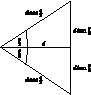
\includegraphics[width=.84\textwidth]{crystal_geometry.pdf}
	\caption[Schematic of the geometry due to the opening angle of the light cone from a \acs{SPDC} source.]{Schematic of the geometry due to the opening angle of the light cone from a \acs{SPDC} source; For a horizontal distance of $d$ from a \acs{SPDC} source, the two frequency-degenerate photons generated from the source will both be at a distance of $d\tan{\frac{\theta}{2}}$ from the horizontal axis, defined by the direction of original beam incident on the crystals.}
	\labelFigure{crystal_geometry}
\end{marginfigure}


\section{Results}
\labelSection{C4_results}
After we performed the coarse alignment procedure described above to a preliminary and satisfactory level, we performed full quantum state tomography for the two-photon, two-qubit polarization-entangled state with the theoretical machinery described by James \etal~\cite{James_2001}. We performed the full set of $16$ polarization measurement settings shown in~\refTableOnly{preliminary}. The coincidence rates were collected over a time interval of \SI{10}{s} for each measurement setting, with a coincidence window of \SI{7}{ns}. For the experimentally generated state $\varrho$,  for each measurement setting and corresponding projector in~\refTableOnly{preliminary}, experimentally we expect to observe the average number of coincidences given by $\nu_v = \expval{\psi_v}{\varrho}$. The set of projectors in the aforesaid table are complete set of measurements, that is, $\varrho$ can be completely and uniquely determined by the said set of measurements. From all $16$ projective measurements, it is possible to recover an estimate of $\varrho$.  Recover a valid density matrix estimate of $\varrho$ (Hermitian, positive etc) the estimate of $\varrho$ is recovered \via maximum likelihood (see~\cite{James_2001} for details). ~\refEquationOnly{preliminary_den} shows the reconstructed density matrix of the polarization entangled-state and~\refFigureOnly{preliminary} shows a graphical representation of this state. 

{
\begin{align}
	\varrho = \mqty(\
		0.43&-0.044-0.042i&0.021-0.061i&-0.14 + 0.32i \\
		-0.044+0.042i&0.013&0.016+0.0089i&-0.0071-0.024i \\
		0.021+0.061i&0.016-0.0892i&0.045&0.020+0.053i \\
		-0.14-0.32i&0.0071+0.024i&0.020-0.053i&0.51
	).
	\labelEquation{preliminary_den}
\end{align}
}

\noindent
The reconstructed state shows a commendable degree of entanglement; It has a fidelity of $F_{\varrho}=0.787\pm 0.0113$ with the maximally entangled state $(\ket{H_1,H_2} - i\ket{V_1,V_2})/\sqrt{2}$. Our measured state also achieves a value of $\ev{S} = 2.344+0.0228$ for the Bell-\acs{CHSH} operator, which represents a violation of the inequality, thus confirming that the state possess non-local correlations. Furthermore, from the density matrix, we can derive physical quantities that give an inkling of the statistical properties of the measured state. One such quantity is the linear entropy, which quantifies the statistical \enquote{mixedness} of the measured state. We measure it to have a value of $S_L= 4/3(1 - \Tr(\varrho^2)) = 0.387+0.0183$. 

\clearpage

\begin{table}[h]
	\centering
	\caption[Measurement settings and coincidence counts for a preliminary tomography analysis of a two-photon polarization state prior to optimization.][6pt]{Measurement settings and coincidence counts for a preliminary tomography analysis of a two-photon polarization state prior to optimization. Coincidence counts, collected over a ten second intervals, for each of the $16$ settings, are sufficient to recover an estimate of the density matrix of the two-qubit polarization state of the two photons. Here, ${\ket{D}\defeq(\ket{H}+\ket{V})/\sqrt{2}}$, ${\ket{L}\defeq(\ket{H}+i\ket{V})/\sqrt{2}}$ and ${\ket{R}\defeq(\ket{H}-i\ket{V})/\sqrt{2}}$}
	\labelTable{preliminary}
	\begin{tabular}{llllllll}
		\toprule
		$m$ & Projector & $h_1$ & $q_1$ & $h_2$ & $q_2$ & $N$ ($10s^{-1}$) \\
		\toprule
		$1$  & $\op{V}\otimes\op{V}$ & $45^{\circ}$   & $0^{\circ}$  & $45^{\circ}$    & $0^{\circ}$   & 2348 \\
		$2$  & $\op{V}\otimes\op{H}$ & $45^{\circ}$   & $0^{\circ}$  & $0^{\circ}$     & $0^{\circ}$   & 24 \\
		$3$  & $\op{H}\otimes\op{H}$ & $0^{\circ}$    & $0^{\circ}$  & $0^{\circ}$     & $0^{\circ}$   & 2410 \\
		$4$  & $\op{H}\otimes\op{V}$ & $0^{\circ}$    & $0^{\circ}$  & $45^{\circ}$    & $0^{\circ}$   & 206 \\
		$5$  & $\op{L}\otimes\op{V}$ & $22.5^{\circ}$ & $0^{\circ}$  & $45^{\circ}$    & $0^{\circ}$   & 720 \\
		$6$  & $\op{L}\otimes\op{H}$ & $22.5^{\circ}$ & $0^{\circ}$  & $0^{\circ}$     & $0^{\circ}$   & 1295 \\
		$7$  & $\op{D}\otimes\op{H}$ & $22.5^{\circ}$ & $45^{\circ}$ & $0^{\circ}$     & $0^{\circ}$   & 1525 \\
		$8$  & $\op{D}\otimes\op{V}$ & $22.5^{\circ}$ & $45^{\circ}$ & $45^{\circ}$    & $0^{\circ}$   & 1346 \\
		$9$  & $\op{D}\otimes\op{L}$ & $22.5^{\circ}$ & $45^{\circ}$ & $22.5^{\circ}$  & $0^{\circ}$   & 2350 \\
		$10$ & $\op{D}\otimes\op{D}$ & $22.5^{\circ}$ & $45^{\circ}$ & $22.5^{\circ}$  & $45^{\circ}$  & 1005 \\
		$11$ & $\op{L}\otimes\op{D}$ & $22.5^{\circ}$ & $0^{\circ}$  & $22.5^{\circ}$  & $45^{\circ}$  & 2132 \\
		$12$ & $\op{V}\otimes\op{D}$ & $45^{\circ}$   & $0^{\circ}$  & $45^{\circ}$    & $45^{\circ}$  & 826 \\
		$13$ & $\op{H}\otimes\op{D}$ & $0^{\circ}$    & $0^{\circ}$  & $0^{\circ}$     & $45^{\circ}$  & 1705 \\
		$14$ & $\op{H}\otimes\op{R}$ & $0^{\circ}$    & $0^{\circ}$  & $0^{\circ}$     & $90^{\circ}$  & 1129 \\
		$15$ & $\op{V}\otimes\op{R}$ & $45^{\circ}$   & $0^{\circ}$  & $45^{\circ}$    & $90^{\circ}$  & 1662 \\
		$16$ & $\op{L}\otimes\op{R}$ & $22.5^{\circ}$ & $0^{\circ}$  & $22.5^{\circ}$  & $90^{\circ}$  & 626 \\
		\toprule
	\end{tabular}
\end{table}

\begin{figure}[h]
    \centering
	\subfloat[\labelFigure{preliminary_re}]
	{
        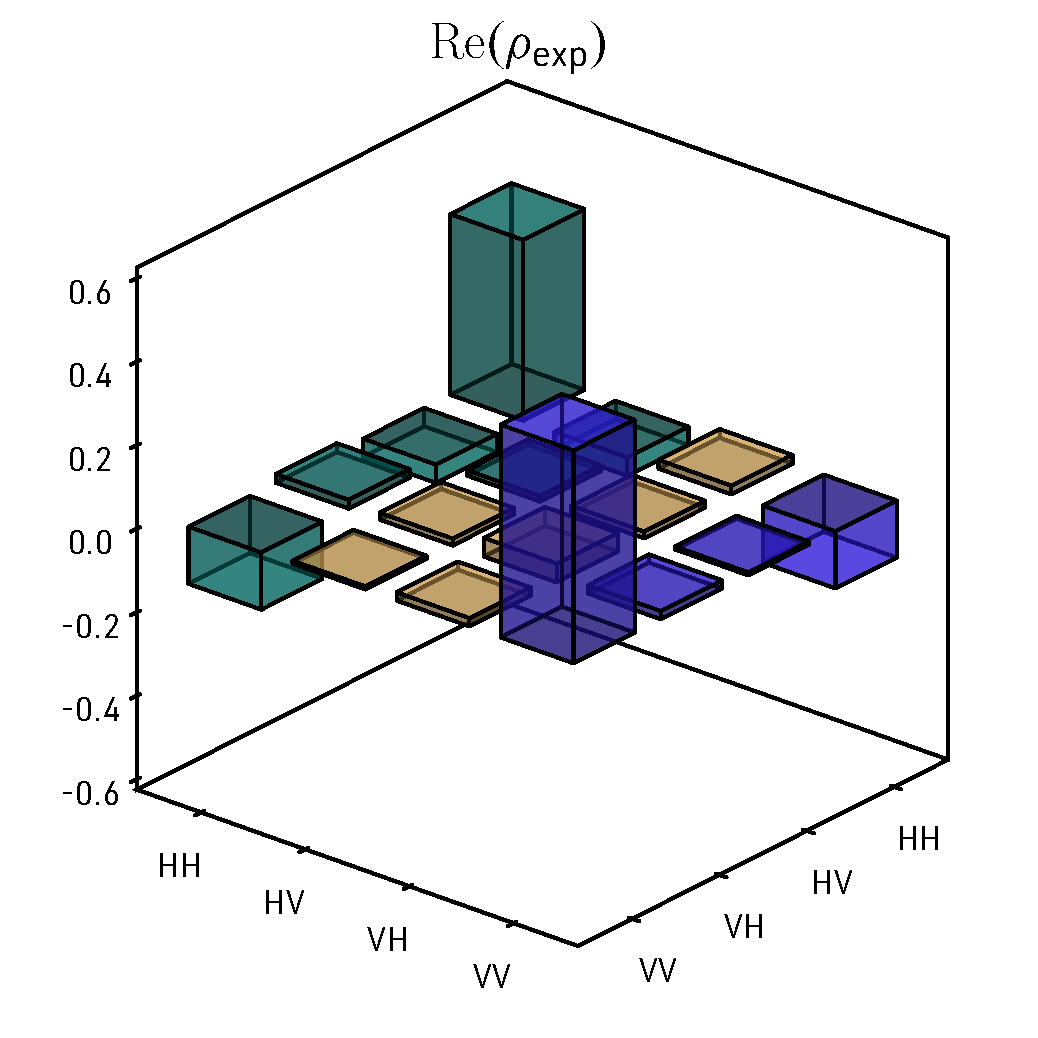
\includegraphics[width=0.5\textwidth]{preliminary_EPR_den_mat_Re.pdf}
	}
	\subfloat[\labelFigure{preliminary_im}]
	{
        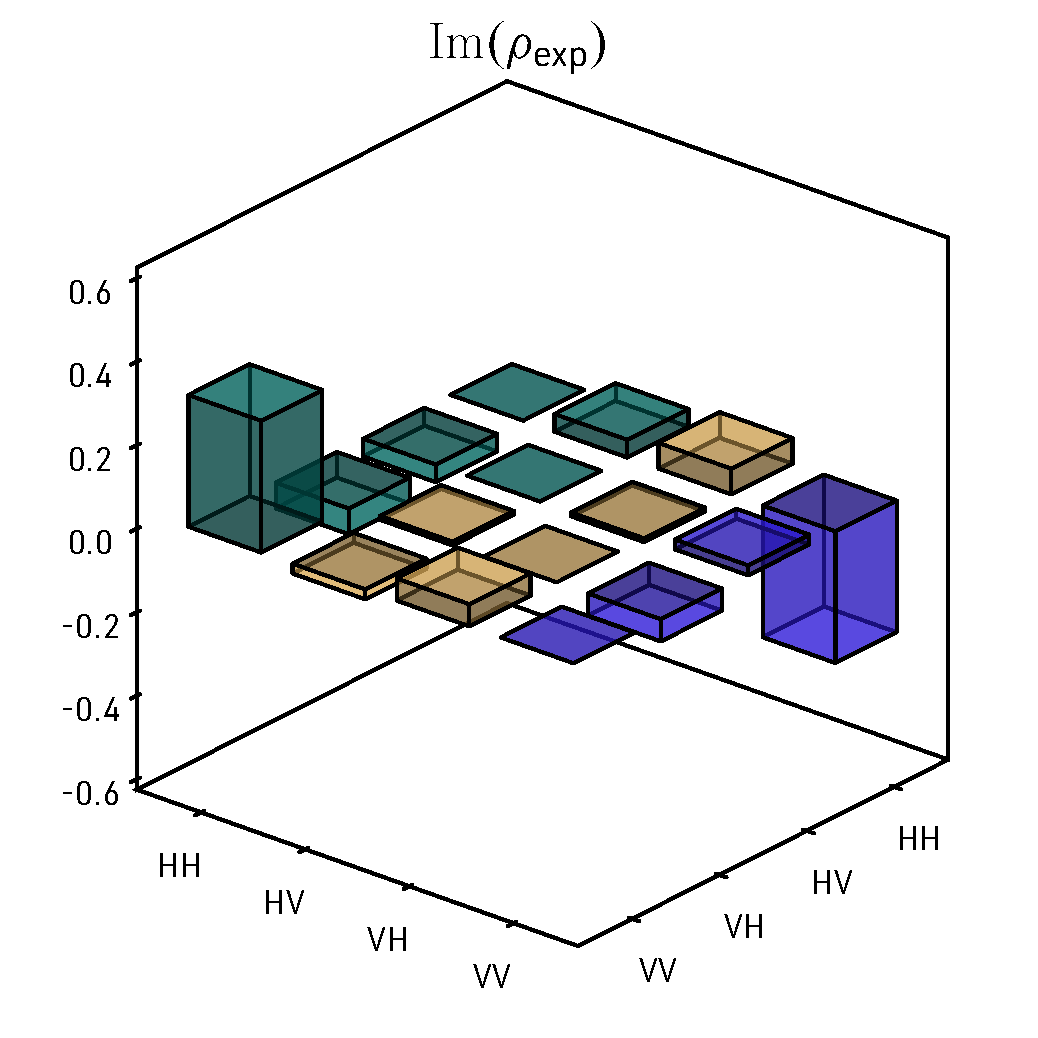
\includegraphics[width=0.5\textwidth]{preliminary_EPR_den_mat_Im.pdf}
	}
	\caption[Density matrix of a state estimated by maximum likelihood tomography from experimental data prior to optimization.]{Density matrix of a state estimated by maximum likelihood tomography prior to optimization, from the experimental data given in~\protect\refTableOnly{preliminary} \textbf{(a)} Real part of the estimate of $\varrho$. \textbf{(b)} Imaginary part of the estimate of $\varrho$.}
	\labelFigure{preliminary}
\end{figure}

\noindent
As also reflected by the graphical representation of the density matrix of this state, this value indicates a considerable amount of mixture present in measured state. The errors of the quantities here were also estimated from a Monte Carlo simulation of $100$ samples with Poisson noise. The values for quantities reported above are not necessarily of low quality; the generated state shows a fidelity of commendable quality, and significant degree of entanglement. However, we had to a reason to suspect that the state generated could be improved. An experiment of a similar kind~\cite{Kwiat_1999}, reports over $140$ coincidence counts per second per milliwatt of pump power over a \SI{5}{\nano\meter} bandwidth and a value of $\ev{S} = 2.700$, thus there is much room for improvement.

\bigskip
\noindent
Next we will describe the optimization procedure followed to improve the quality of the state generated in the experiment, and the subsequent result. Optimization is with respect to some utility function, and what will be described here is not necessarily a procedure suitable in all circumstances, and definitively imperfect. An imperative of uttermost practical importance to our experiment, was the tuning of the value of $\phi$ in the state $\ket{H_1,H_2} + e^{i\phi}\ket{V_2,V_2}$ generated by the \acs{SPDC} source. 

\clearpage
\noindent
As it can be inferred from the preliminary results, for that particular state, which has a significant fidelity with the state $\ket{H_1,H_2} - i\ket{V_1,V_2}$, the value of $\phi$ can be crudely inferred to take on a value $\phi=\pi$. We seek to generate one of the four Bell states:

\begin{align}
	\labelEquation{bell_states}
	\ket{\Phi^+}   &= \frac{1}{\sqrt{2}} \left(\ket{H_1,H_2} + \ket{V_1,V_2}\right), \nonumber \\
	\ket{\Phi^-}   &= \frac{1}{\sqrt{2}} \left(\ket{H_1,H_2} - \ket{V_1,V_2}\right),\nonumber \\
	\ket{\Psi^{+}} &= \frac{1}{\sqrt{2}} \left(\ket{H_1,V_2} + \ket{V_1,H_2}\right), \nonumber \\
	\ket{\Psi^{-}} &= \frac{1}{\sqrt{2}} \left(\ket{H_1,V_2} - \ket{V_1,H_2}\right).
\end{align}

\noindent
This imperative is once again motivated by the end goal of ultimately generating a three qubit \acs{GHZ} state. Thus, with this end in view, it is more experimentally convenient if we were to generate either one of the first two Bell states in~\refEquationOnly{bell_states}. In any case, our \acs{SPDC} source alone is limited to the generation of these two particular Bell states\footnote[][-10pt]{All four Bell states are equivalent up to some local unitary operation, for instance, if our \acs{SPDC} source generates the states $\ket{H_1,H_2}\pm\ket{V_1,V_2}$, an extra \acs{HWP} in the second arm that interchanges $H$ and $V$ (rotated $45^{\circ}$ counterclockwise to its fast-axis), prepares $\ket{H_1,V_2}\pm\ket{V_1,H_2}$. Similarly, the unitary operator $U = \mathds{1} \otimes S$, where $S=\diag(1, i)$, acting on $\ket{H,H}\pm i\ket{V_1,V_1}$, prepares $\ket{H_1,H_2}\pm\ket{V_1,V_1}$.}. We chose to optimize for the second Bell state, the optimization procedure for this particular state is guarded by the following observations.

\bigskip
\noindent
Consider one of the projectors from tomography analysis, $P_{DD} = \op{D_1}\otimes\op{D_2}$ where $\ket{D} = (\ket{H} + \ket{V})/\sqrt{2}$. Calculating the expectation value of the projector\footnote[][40pt]{This expectation value is related to the probability of a getting an outcome associated with the projector upon performing the projective measurement on $\ket{\Phi^{-}}$.} with respect to the state $\ket{\Phi^{-}}$ in ~\refEquationOnly{bell_states}, we observe that (omitting normalization constants):

\begin{align}
	\labelEquation{obs_1}
	&\ev{P_{DD}}{\Phi^{-}} = \ev{(\ketbra{D_1}{D_1} \otimes \
	\ketbra{D_2}{D_2})}{\Phi^{-}} \nonumber, \\
	&=\abs{\bra{H}\ket{D}}^4 - \
	\abs{\braket{D}{H}\braket{V}{D}}^2 - \
	\abs{\braket{D}{H}\braket{V}{D}}^2 + \
	\abs{\bra{V}\ket{D}}^4 \nonumber ,\\
	&= \left(\frac{1}{\sqrt{2}}\right)^4 - \left(\frac{1}{\sqrt{2}}\right)^4 - \left(\frac{1}{\sqrt{2}}\right)^4 + \left(\frac{1}{\sqrt{2}}\right)^4 \nonumber ,\\
	&= 0.
\end{align}

\noindent
Similarly, the projector $P_{LR} = \op{L_1}\otimes\op{R_2}$, where $\ket{L/R} = (\ket{H} \pm i \ket{V})/\sqrt{2}$ gives:

\begin{align}
	\labelEquation{obs_2}
	&\ev{P_{LR}}{\Phi^{-}} = \ev{(\ketbra{L_1}{L_1} \otimes \
	\ketbra{R_2}{R_2})}{\Phi^{-}} \nonumber, \\
	&=\abs{\braket{H}{L} \braket{R}{H}}^2 - \
	\braket{H}{L}\braket{L}{H}\braket{H}{R}\braket{R}{V} \nonumber, \\
	&\quad-\braket{V}{L}\braket{L}{H}\braket{V}{R}\braket{R}{H} + \
	\abs{\braket{V}{L} \braket{R}{V}}^2 \nonumber, \\
	&= \left(\frac{1}{\sqrt{2}}\right)^4 - \left(\frac{1}{\sqrt{2}}\right)^4 - \left(\frac{1}{\sqrt{2}}\right)^4 + \left(\frac{1}{\sqrt{2}}\right)^4 \nonumber, \\
	&= 0. 
\end{align}

\noindent
Aided by the above observations, we conjure up a procedure to optimize for the state $\ket{\Phi^-}$:

\begin{itemize}
	\item[\emph{Primo}] Set the polarization analysis optics to project out $\ket{H_1,H_2}$ and maximize the corresponding coincidence counts, typically achieved by fine adjustments to using the $z$-dial on the kinematic mount that holds the \acs{BBO} crystals, which tilts the crystals with respect to the $z$-$x$ plane (left-handed Cartesian coordinate system). Similarly, maximize the coincidence counts for the projection of $\ket{V_1,V_2}$, achieved by fine adjustments to the dials on the rotation stage at the bottom of the kinematic mount, which rotate the crystals about to the $z$-axis. \item[\emph{Secondo}] Set the polarization analysis optics to project out $\ket{D_1,D_2}$ and minimize the corresponding coincidence counts, which we achieved by rotating the crystals with respect to $y$-axis with the radial dial on the kinematic mount. Similarly, set the polarization analysis optics to project out $\ket{L_1,R_2}$ and minimize the corresponding coincidence counts, by using the $x$-$y$ axis dials on either side of the kinematic mount.
	\item[\emph{Terzo}] We go through several iterations of this process, and roughly equalize the two coincidence counts observed for $\ket{H_1,H_2}$ and $\ket{V_1,V_2}$, while minimizing the ones observed for $\ket{D_1,D_2}$ and $\ket{L_1,R_2}$.
\end{itemize}

\noindent
While iterating the steps of the above procedure, one eventually reaches a point where additional iterations have non-desirable results; The coincidence counts for $\ket{D_1,D_2}$ and $\ket{L_1,R_2}$ reach some local minimum (typically around $30s^{-1}$) and start increasing again, or the counts for $\ket{H_1,H_2}$ and $\ket{V_1,V_2}$ are no longer equal. At this point we halt and take the previous iteration to be optimal. Physically, the optimization procedure is changing the opening directions of the two light cones emerging from the \acs{BBO} crystals such that the collection optics in our experiment can access as much of the light cones as possible, and as close as possible to diametrically-opposed regions of indistinguishability. The measurement results after several iterations of this process are shown in ~\refTableOnly{tomo_analysis} and the corresponding graphical representation of the reconstructed density matrix shown in~\refFigureOnly{2q_tomo}, where the corresponding density matrix for the two-photon state is given by

\begin{align}
	\labelEquation{epr_density}
	\varrho = \mqty(
		0.49&0.028+0.033i&0.017-0.025i&-0.41+0.054i \\
		0.028-0.033i&0.0074&-0.0019+0.0017i&0.0011+0.023i \\
		0.017+0.025i&-0.0019-0.0017i&0.0074&-0.034-0.042i \\
		-0.41-0.054i&0.0011-0.023i&-0.034+0.042i&0.49 \\
	).
\end{align}

\noindent
From the above density matrix and its graphical representation, in comparison to the earlier reconstruction in ~\refFigureOnly{preliminary}, we note a few conspicuous differences. The populations of horizontally-and vertically-polarized photons are equalized in the optimized measured state\footnote[][-10pt]{Represented by the diagonal element on the top-left and diagonal element bottom-right respectively.}.  Likewise, the coherences\footnote[][20pt]{Represented by the off-diagonal elements. For this particular instance, the entries on the bottom left and top right.} between these two populations are equalized, and have a close resemblance to the coherences of the Bell state $\ket{\Phi^{-}}$; the fidelity between the measured state and the aforementioned state is $F_\varrho=0.902 \pm 0.00588$. Furthermore, there is an improvement of the other previously reported physical quantities; The measured state a violates a Bell-\acs{CHSH} inequality, attaining a value of $\ev{S} = 2.594\pm0.0153$. 

\bigskip
\noindent
Lastly, the linear entropy of the above state has a value of $S_L=0.211\pm0.0134$, which reflects a decrease in the \enquote{mixedness} of the state, in comparison to the earlier reconstruction. The errors in these quantities were estimated from a Monte Carlo simulation of $100$ samples with Poissonian noise on the count statistics\footnote[][-40pt]{This is because due to the probabilistic nature of \acs{SPDC}, the number of $n$ discrete photon pairs that arrive at the detectors for given a collection time interval $\Delta t$ follows a Poissonian probability distribution $\text{Pois}(\lambda = n \Delta t)$.}.

\clearpage

\begin{table}[t!]
	\centering
	\caption[Measurement settings and doublce coincidence counts for a tomography analysis of a two-photon polarization state after optimization.][6pt]{Measurement settings and coincidence counts for a tomography analysis of a two-photon polarization state after optimization. Coincidence counts, collected over a ten second intervals, for each of the $16$ settings, are sufficient to recover an estimate of (reduced) density matrix of the two-qubit polarization state of the two photons. Here, ${\ket{D}\defeq(\ket{H}+\ket{V})/\sqrt{2}}$, ${\ket{L}\defeq(\ket{H}+i\ket{V})/\sqrt{2}}$ and ${\ket{R}\defeq(\ket{H}-i\ket{V})/\sqrt{2}}$.}
	\labelTable{tomo_analysis}
	\begin{tabular}{llllllll}
		\toprule
		$m$ & Projector & $h_1$ & $q_1$ & $h_2$ & $q_2$ & $N$ ($10s^{-1}$) \\
		\toprule
		$1$  & $\op{V}\otimes\op{V}$ & $45^{\circ}$   & $0^{\circ}$  & $45^{\circ}$    & $0^{\circ}$   & 2738(83) \\
		$2$  & $\op{V}\otimes\op{H}$ & $45^{\circ}$   & $0^{\circ}$  & $0^{\circ}$     & $0^{\circ}$   & 33(5) \\
		$3$  & $\op{H}\otimes\op{H}$ & $0^{\circ}$    & $0^{\circ}$  & $0^{\circ}$     & $0^{\circ}$   & 2718(69) \\
		$4$  & $\op{H}\otimes\op{V}$ & $0^{\circ}$    & $0^{\circ}$  & $45^{\circ}$    & $0^{\circ}$   & 35(2) \\
		$5$  & $\op{L}\otimes\op{V}$ & $22.5^{\circ}$ & $0^{\circ}$  & $45^{\circ}$    & $0^{\circ}$   & 1256(14) \\
		$6$  & $\op{L}\otimes\op{H}$ & $22.5^{\circ}$ & $0^{\circ}$  & $0^{\circ}$     & $0^{\circ}$   & 1492(40) \\
		$7$  & $\op{D}\otimes\op{H}$ & $22.5^{\circ}$ & $45^{\circ}$ & $0^{\circ}$     & $0^{\circ}$   & 1470(23) \\
		$8$  & $\op{D}\otimes\op{V}$ & $22.5^{\circ}$ & $45^{\circ}$ & $45^{\circ}$    & $0^{\circ}$   & 1479(26) \\
		$9$  & $\op{D}\otimes\op{L}$ & $22.5^{\circ}$ & $45^{\circ}$ & $22.5^{\circ}$  & $0^{\circ}$   & 1434(46) \\
		$10$ & $\op{D}\otimes\op{D}$ & $22.5^{\circ}$ & $45^{\circ}$ & $22.5^{\circ}$  & $45^{\circ}$  & 284(15) \\
		$11$ & $\op{L}\otimes\op{D}$ & $22.5^{\circ}$ & $0^{\circ}$  & $22.5^{\circ}$  & $45^{\circ}$  & 1614(31) \\
		$12$ & $\op{V}\otimes\op{D}$ & $45^{\circ}$   & $0^{\circ}$  & $45^{\circ}$    & $45^{\circ}$  & 1549(31)\\
		$13$ & $\op{H}\otimes\op{D}$ & $0^{\circ}$    & $0^{\circ}$  & $0^{\circ}$     & $45^{\circ}$  & 1079(11) \\
		$14$ & $\op{H}\otimes\op{R}$ & $0^{\circ}$    & $0^{\circ}$  & $0^{\circ}$     & $90^{\circ}$  & 1661(46) \\
		$15$ & $\op{V}\otimes\op{R}$ & $45^{\circ}$   & $0^{\circ}$  & $45^{\circ}$    & $90^{\circ}$  & 1159(24) \\
		$16$ & $\op{L}\otimes\op{R}$ & $22.5^{\circ}$ & $0^{\circ}$  & $22.5^{\circ}$  & $90^{\circ}$  & 254(12) \\
		\toprule
	\end{tabular}
\end{table}

\begin{figure}[t!]
    \centering
	\subfloat[\labelFigure{epr_den_mat_real}]
	{ %
        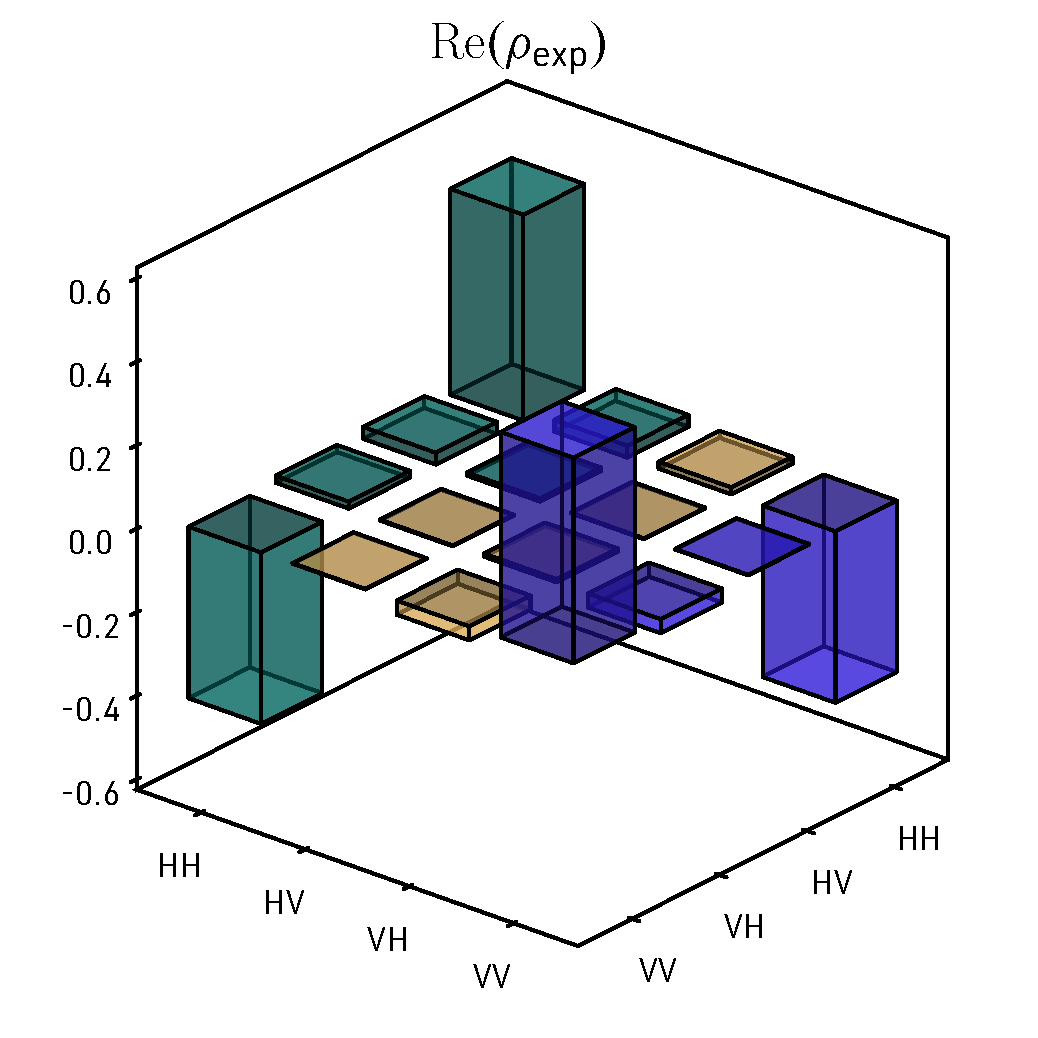
\includegraphics[width=0.5\textwidth]{EPR_den_mat_Re.pdf}
	}
	\subfloat[\labelFigure{epr_den_mat_img}]
	{ %
        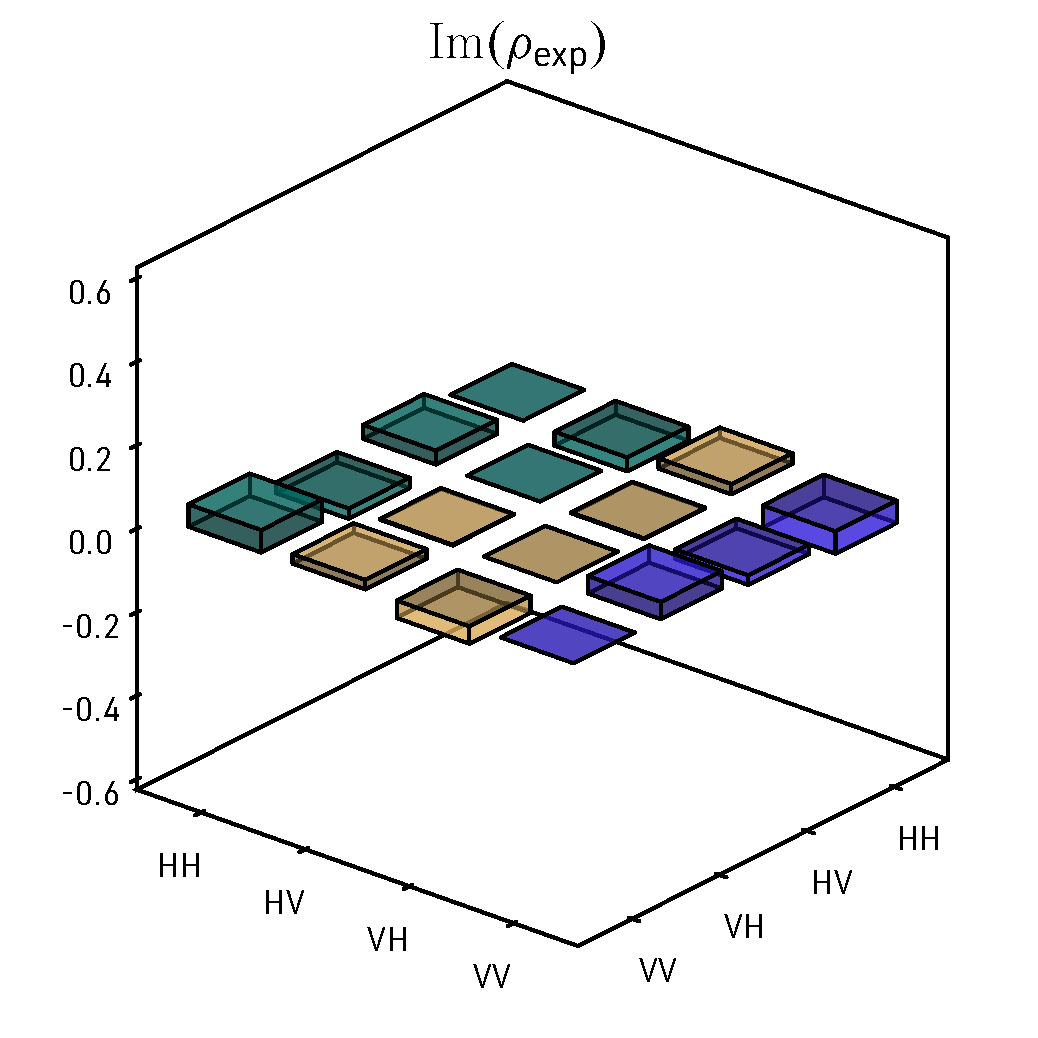
\includegraphics[width=0.5\textwidth]{EPR_den_mat_Im.pdf}
	}
\caption[Density matrix of a state estimated by maximum likelihood tomography from experimental data after optimization.]{Density matrix of a state estimated by maximum likelihood tomography from the experimental data given in~\protect\refTableOnly{tomo_analysis} after optimization. \textbf{(a)} Real part of the estimate of $\varrho$. \textbf{(b)} Imaginary part of the estimate of $\varrho$.}
	\labelFigure{2q_tomo}
\end{figure}

\noindent
Alas, while the above results improve over the preliminary results and are in good agreement with expected state $\ket{H_1,H_2} - \ket{V_1,V_2}$, unwanted artefacts such as the apparent loss in the coherences of the two orthogonal polarizations and a small, non-negligible mixedness of the state, in the reconstructed state still persist. The origins of some of these unwanted artefacts can be attributed to systematic errors, such as those stemming from efficiencies of the various optical components in the experiment\footnote[][-30pt]{PBS transmission and reflection efficiencies, photon detector efficiency and their coupling efficiency to optical fibres, collection efficiencies etc.}. 

\bigskip
\noindent
While the origins of the loss of coherences are often attributable to the many decoherence mechanisms of polarization-entangled sources, which vary from source to source and dependent on nature and application of the experiment at hand. We will briefly outline the two decoherence mechanisms that are relevant to our application, following references~\cite{Akselrod_2007, Akselrod_err_2007, Baek_2008, Rangarajan_2009}.

\clearpage
\noindent
An ideal process of type-I \acs{SPDC} has stringent phase matching conditions; for a pump photon incident on a crystal down converts to two photons, a signal and an idler photon, with the same polarization. The entire process must both conserve momentum and energy, which give rise to the aforementioned conditions:

\begin{align}
	\labelEquation{phase_match}
	\vec{k}_i + \vec{k}_s = \vec{k}_p, \nonumber \\
	\omega_i + \omega_s = \omega_p,
\end{align}

\noindent
where $\vec{k}$ and $\omega$ are the wave vector and frequency of the photon respectively. The subscripts $i$, $s$ and $p$ refer to the idler, signal and pump photon respectively. For a frequency degenerate type-I \acs{SPDC} process, the idler and signal photons have half the frequency of the pump photon individually. In an ideal experiment, one expects the phase-matching conditions to be perfectly satisfied, in an actual experiment this is not the case. In reality, there is often a phase mismatch, which enters into~\refEquationOnly{phase_match} \via an additional effective wave vector $\vec{\Delta}$, which has a non-trivial effect on the spectral properties of the process. 

\begin{align}
	\labelEquation{phase_mismatch}
	\vec{k}_i + \vec{k}_s + \vec{\Delta} = \vec{k}_p.
\end{align}

\noindent
Ideally, for a type-I non-collinear degenerate \acs{SPDC} process, only frequency-degenerate photon pairs are emitted at the emission angle of the light cones. However, due to the phase mismatch, it is possible for the process to also produce non-degenerate frequency photons pairs. The emission angles of the non-degenerate pairs will not always be asymmetric around pump beam; the findings in Ref.~\cite{Baek_2008} report the production of non-degenerate pairs at \SI{662.2}{\nano\meter} (signal photon) and \SI{747.3}{\nano\meter} (idler photon) respectively, with the signal photon within the collection angle of their system (around $3^{\circ}$), while the idler photon falls outside this collection angle, hence does not contributing to the single photon rates. 

\bigskip
\noindent
The said effect produces spectral profiles for both signal and idler photons that are asymmetric around the degenerate frequency. The result of this spectral profile asymmetry along with the geometry of a experiment, have a bearing on the two-photon joint spectra which determines the coincidence counts. Baek and Kim ~\cite{Baek_2008} show that the joint spectra is significantly reduced in comparison to the spectral profile of the signal/idler photon pairs, and limited by the collection angles in their experiment, $2.95^{\circ} - 3.17^{\circ}$; this collection range does not collect one of the photons from a non-degenerate pair.  As a result, the two-photon spectra can also have asymmetric spectral profile around the degenerate frequency, which can be significantly altered by small alignment errors. 


\bigskip
\noindent
A way to compensate for this spectral asymmetry is by way of spectral filtering over the bandwidth of a narrow bandwidth filter around the degenerate frequency, the spectral profiles of the idler and signal photons, and consequently two-photon joint spectra are made more similar to one another, by effectively filtering out the unwanted non-degenerate photon pairs. This method of compensation comes at the expense of collection efficiency of the experiment. The spectral filters in our experiment have quite a broad bandwidth, centred at \SI{800}{\nano\meter} with a \acs{FWHM} of \SI{40}{\nano\meter}, thus it is not far-fetched to suspect the presence of non-degenerate photon pairs, which is by evidenced by the significantly high single count rate in comparison to coincidence rate (by roughly a scale $\sim 0.3$). 

\clearpage
\noindent
We attempted to use narrow bandwidth filters, centred at $\SI{810}{\nano\meter}$ with a \acs{FWHM} of \SI{10}{\nano\meter}, which did not improve the results by much, upon inspection, we found that when filtering a white light source\footnote{Fianium WhiteLase micro with spectrum $<$\SI{450}{nm} to $>$\SI{2000}{nm} with a pulse width of $\approx$\SI{6}{ps} and a repetition rate of \SI{20}{MHz}.} the two filters had non-overlapping regions of considerable size in their spectral profiles. One of the interference filters was not centred at \SI{810}{\nano\meter} (as indicated by the manufacturer) but slightly higher, which for the interim explains why the results did not improve by much.

\bigskip
\noindent
Another dominant decoherence mechanism, particularly for a paired-\acs{BBO} type-I \acs{SPDC} source, is one that degrades the temporal indistinguishability of the down converted photons. Crudely represented, the two crystals having finite thickness, means the two down-conversion processes in the two crystals will occur at slightly different times (order of femtoseconds). Over the thickness of the crystals, both birefringent and dispersive effects influence the group velocities of both signal and idler photons, and subsequently their emission times from the two crystals. If the assumption is that two down-conversion processes take place at halfway the length of each crystal, then time taken by the signal and idler photons to traverse the length $L$ of the two crystals, can be calculated as follows~\cite{Rangarajan_2009}.  For photons down converted in the first crystal:

\begin{itemize}
	\item[\emph{Primo}] A pump photon will traverse half of the length of the first crystal where it is extraordinary polarized, after which it down converts resulting in a polarization perpendicular to the original and hence ordinary polarized. 
	\item[\emph{Secondo}] The resulting signal/idler photon will traverse the second half of the first crystal ordinary polarized.
	\item[\emph{Terzo}] After exiting the first crystal, the signal/idler photon will traverse the full length of the second crystal extraordinary polarized.
\end{itemize}

\noindent
The time spent by a signal photon in each of the three stages above depends on the refractive-index-dependent group velocities of ordinary and extraordinary photons in the two crystals and the length $L$:

\begin{align}
	t_s &= \frac{L}{2V^{e}_g(\omega_p)} + \frac{L}{2V^{o}_g(\omega_s)} +
	\frac{L}{V^{e}(\omega_s)},
\end{align}

\noindent
the reasoning is similar for photons down converted in the second crystal, and gives: 

\begin{align}
	t'_s &= \frac{L}{V^{o}_g(\omega_p)} + \frac{L}{2V^{e}_g(\omega_p)} + \frac{L}{2V^{o}_g(\omega_s)},
\end{align}

and the net delay $\Delta t_s$ between the two down conversion processes is given by

\begin{align}
	\Delta t_s  = t'_s - t_s = L \left(\frac{1}{V^{o}_g(\omega_p)} - \frac{1}{V^{e}_g(\omega_s)} \right).
\end{align}

\noindent
The above time difference leads to the degradation of the temporal indistinguishability between the two light cones; photons belonging to one light cone will be delayed by $\Delta t_{s/i}$ relative to the photons from the other light cone. 

\clearpage
\noindent
Rangarajan~\etal~\cite{Rangarajan_2009} derive an expression for the density matrix of the two-photon down converted state with such a delay:

\begin{align}
	\varrho'  = \frac{1}{2} \mqty(
		1 & 0 & 0 & \nu(\Delta t_s, \Delta t_i) \\
		0 & 0 & 0 & 0 \\
		0 & 0 & 0 & 0 \\
		\nu^*(\Delta t_s, \Delta t_i) & 0 & 0 & 1
	),
\end{align}

\noindent
where $\nu(\Delta_s, \Delta_i)$ is dependent on the two-photon joint spectra. As expected, we note that this decoherence mechanism has no effect on the two populations but only affects the coherence between the two polarizations. Refs.~\cite{Akselrod_2007, Akselrod_err_2007, Rangarajan_2009} recommended the use of birefringent crystals, with the same but opposite time delay between extraordinary and ordinary components of the pump photons, to pre(post)compensate for the delay between the emission-times of the two down conversion processes. With use of such techniques, they were able to state fidelities in excess of $0.977$.

\section{Concluding remarks}
\labelSection{C4_concluding_remarks}
In this chapter, we described and conducted an experiment based on \acs{SPDC}, generating a two-photon two-qubit polarization-entangled state. The generated state is fully characterized through \acs{QST}, recovering its density matrix, from which other physical quantities of interest, such as those quantifying the degree of entanglement possessed by the state can be derived from. The \acs{SPDC} source is optimized, with a rule of thumb procedure described in the text, to generate one of the Bell states ($\ket{\Phi^{-}}$). We repeat this process until we achieve a fidelity of $0.90$. In comparison to similar demonstrations in the current literature, which can achieve fidelities in access of $0.97$, this is a relatively is low fidelity, nevertheless the obtained result is satisfactory to our experimental needs. Lastly, we briefly outlined a description of the two decoherence mechanisms for paired \acs{BBO} type-I non-collinear \acs{SPDC} and how these maybe counteracted to improve the fidelity of the generated polarization-entangled state. In the chapter that follows, we will describe how the polarization-entangled state generated by this Bell-state photon pair source may be extended to accommodate an additional qubit through a different \acs{DOF}.
